% Drawing 142/03-1 -- folder 142, batch 03, archive page 49 (PDF page 50).
% Transcription: une sphère, pôles $P^{+}$ en haut et $P^{-}$ en bas, l'équateur $\Sigma_{\mathbf{R}}$ portant les trois trous $R_0$, $R_1$, $R_\infty$, chacun entouré de son petit cercle $U_i$ marqué des points $R_i^{\pm}$, $S_i^{\pm}$ et des arcs $a_i^{++}, a_i^{+-}, \dots$ ; sur l'équateur les points $Q_0$, $Q_1$, $Q_\infty$ et les arcs orientés $b_i^{\pm}$ ; des pôles partent les méridiens portant les arcs $c_i^{\pm}$ (vers les $Q_i$) et $d_i^{\pm}$ (vers les $S_i$), en traits pleins ou pointillés selon l'hémisphère.
% Kind: sphere with poles, meridians, equatorial vertices and holes. Method 2 (schematic redraw from the facsimile). Status: partial.
% Notes: Pencil outline; P^+ and P^-; on the equator Q_1, Q_infty, Q_0 and the three holes R_0, R_infty, R_1, each in its small circle U_i with R_i^+-, S_i^+-; the oriented arcs b_i^+- along the equator (dotted at the back), the meridians d_i^+- (to the S_i) and c_i^+- (to the Q_i), solid or dotted as on the page. The many small labels a_i^{++}, a_i^{+-}, ... round the circles are overinked; only the legible ones are placed. The circle round R_1 is at the right edge of the figure and partly cut by the crop of his own strokes.
% Coordinates: 1 unit = 1 mm = 1/100 of the crop width (bbox in page fractions: [0.13, 0.08, 0.53, 0.43]).
% Redrawn by Claude (claude-opus-5-5), issue #73, 2026-11-07; not checked by a human; not compiled (no TeX in the session).
% Rights: reproduces part of the work -- behind RENDER_TRANSCRIPTS, never published by itself.
\documentclass[tikz,border=3pt]{standalone}
\usepackage{amsmath,amssymb}
\usetikzlibrary{patterns,arrows.meta}
\tikzset{pencil/.style={black!45}, struck/.style={black!35}, mark/.style={circle,draw,inner sep=1.3pt}, pt/.style={circle,fill,inner sep=0.9pt}, opt/.style={circle,draw,fill=white,inner sep=1.1pt}}
\begin{document}
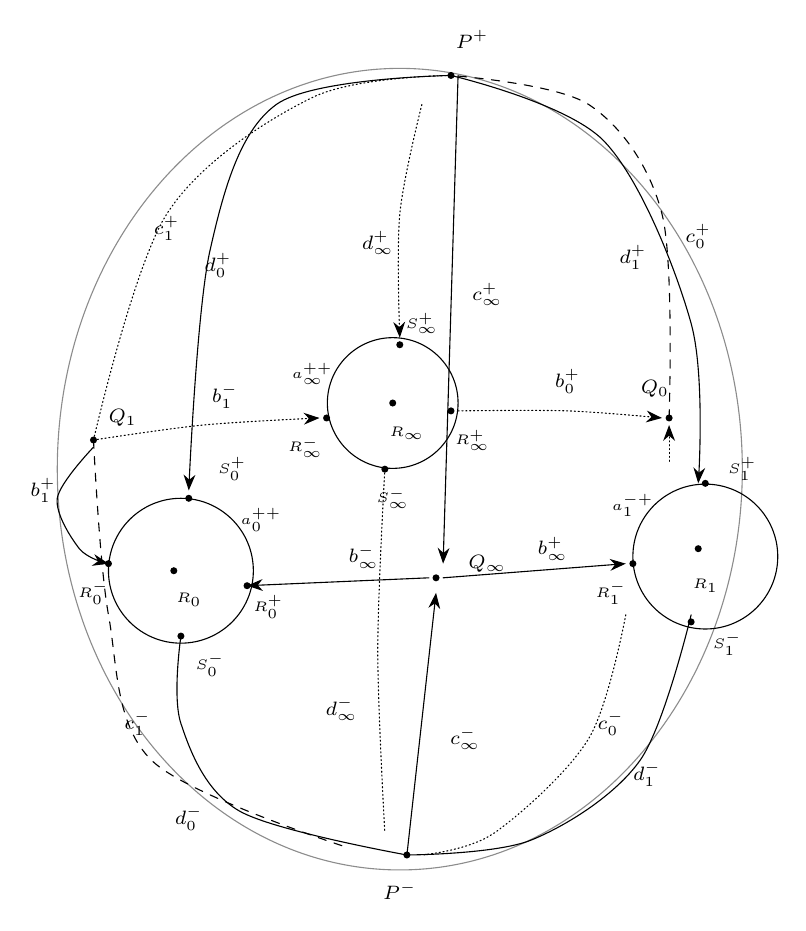
\begin{tikzpicture}[x=1mm,y=1mm,line cap=round,line join=round,font=\scriptsize]
\draw[pencil] (48.1,-69.4) ellipse[x radius=43.5, y radius=50.9];
\node[pt] at (54.6,-19.4) {};
\node[pt] at (49,-118.4) {};
\node[pt] at (9.2,-65.7) {};
\node[pt] at (52.7,-83.2) {};
\node[pt] at (82.3,-62.9) {};
\draw[-{Stealth[length=2mm]}] plot[smooth, tension=0.55] coordinates {(54.6,-19.4) (32.4,-23.1) (24,-41.6) (21.3,-72.1)};
\draw[-{Stealth[length=2mm]}] plot[smooth, tension=0.55] coordinates {(54.6,-19.4) (74,-27.7) (85.1,-50.9) (86,-71.2)};
\draw[-{Stealth[length=2mm]}] (55.5,-19.4) -- (53.6,-81.4);
\draw[-{Stealth[length=2mm]}] (49,-118.4) -- (52.7,-85.1);
\draw[densely dotted,-{Stealth[length=2mm]}] plot[smooth, tension=0.55] coordinates {(50.9,-23.1) (48.1,-37) (48.1,-52.7)};
\draw[densely dotted] plot[smooth, tension=0.55] coordinates {(46.2,-69.4) (45.3,-92.5) (46.2,-115.6)};
\draw plot[smooth, tension=0.55] coordinates {(20.3,-90.6) (20.3,-101.7) (27.7,-112.8) (49,-118.4)};
\draw plot[smooth, tension=0.55] coordinates {(85.1,-87.9) (78.6,-106.4) (64.8,-116.5) (49,-118.4)};
\draw[densely dotted] plot[smooth, tension=0.55] coordinates {(9.2,-65.7) (18.5,-37) (37,-22.2) (54.6,-19.4)};
\draw[dashed] plot[smooth, tension=0.55] coordinates {(82.3,-62.9) (81.4,-37) (72.1,-23.1) (54.6,-19.4)};
\draw[dashed] plot[smooth, tension=0.55] coordinates {(9.2,-65.7) (11.1,-87.9) (16.6,-106.4) (41.6,-117.5)};
\draw[densely dotted] plot[smooth, tension=0.55] coordinates {(76.8,-87.9) (72.1,-103.6) (60.1,-115.6) (50.9,-118.4)};
\draw[densely dotted,-{Stealth[length=2mm]}] plot[smooth, tension=0.55] coordinates {(9.2,-65.7) (23.1,-63.8) (37.9,-62.9)};
\draw[densely dotted,-{Stealth[length=2mm]}] plot[smooth, tension=0.55] coordinates {(55.5,-62) (69.4,-62) (81.4,-62.9)};
\draw[densely dotted,-{Stealth[length=2mm]}] (82.3,-68.4) -- (82.3,-63.8);
\draw[-{Stealth[length=2mm]}] (51.8,-83.2) -- (28.7,-84.2);
\draw[-{Stealth[length=2mm]}] (53.6,-83.2) -- (76.8,-81.4);
\draw[-{Stealth[length=2mm]}] plot[smooth, tension=0.55] coordinates {(9.2,-66.6) (4.6,-73.1) (7.4,-79.5) (11.1,-81.4)};
\draw (20.3,-82.3) ellipse[x radius=9.2, y radius=9.2];
\draw (47.2,-61) ellipse[x radius=8.3, y radius=8.3];
\draw (86.9,-80.5) ellipse[x radius=9.2, y radius=9.2];
\node[pt] at (19.4,-82.3) {};
\node[pt] at (47.2,-61) {};
\node[pt] at (86,-79.5) {};
\node[pt] at (11.1,-81.4) {};
\node[pt] at (28.7,-84.2) {};
\node[pt] at (21.3,-73.1) {};
\node[pt] at (20.3,-90.6) {};
\node[pt] at (38.8,-62.9) {};
\node[pt] at (54.6,-62) {};
\node[pt] at (48.1,-53.6) {};
\node[pt] at (46.2,-69.4) {};
\node[pt] at (77.7,-81.4) {};
\node[pt] at (86.9,-71.2) {};
\node[pt] at (85.1,-88.8) {};
\node[inner sep=1pt] at (57.3,-14.8) {\scriptsize $P^{+}$};
\node[inner sep=1pt] at (48.1,-123) {\scriptsize $P^{-}$};
\node[inner sep=1pt] at (12.9,-62.9) {\scriptsize $Q_1$};
\node[inner sep=1pt] at (80.5,-59.2) {\scriptsize $Q_0$};
\node[inner sep=1pt] at (59.2,-81.4) {\scriptsize $Q_\infty$};
\node[inner sep=1pt] at (25,-43.5) {\scriptsize $d_0^{+}$};
\node[inner sep=1pt] at (45.3,-40.7) {\scriptsize $d_\infty^{+}$};
\node[inner sep=1pt] at (59.2,-47.2) {\scriptsize $c_\infty^{+}$};
\node[inner sep=1pt] at (77.7,-42.5) {\scriptsize $d_1^{+}$};
\node[inner sep=1pt] at (86,-39.8) {\scriptsize $c_0^{+}$};
\node[inner sep=1pt] at (18.5,-38.8) {\scriptsize $c_1^{+}$};
\node[inner sep=1pt] at (25.9,-60.1) {\scriptsize $b_1^{-}$};
\node[inner sep=1pt] at (69.4,-58.3) {\scriptsize $b_0^{+}$};
\node[inner sep=1pt] at (2.8,-72.1) {\scriptsize $b_1^{+}$};
\node[inner sep=1pt] at (43.5,-80.5) {\scriptsize $b_\infty^{-}$};
\node[inner sep=1pt] at (67.5,-79.5) {\scriptsize $b_\infty^{+}$};
\node[inner sep=1pt] at (40.7,-99.9) {\scriptsize $d_\infty^{-}$};
\node[inner sep=1pt] at (56.4,-103.6) {\scriptsize $c_\infty^{-}$};
\node[inner sep=1pt] at (74.9,-101.7) {\scriptsize $c_0^{-}$};
\node[inner sep=1pt] at (14.8,-101.7) {\scriptsize $c_1^{-}$};
\node[inner sep=1pt] at (21.3,-113.8) {\scriptsize $d_0^{-}$};
\node[inner sep=1pt] at (79.5,-108.2) {\scriptsize $d_1^{-}$};
\node[inner sep=1pt] at (21.3,-86) {\tiny $R_0$};
\node[inner sep=1pt] at (49,-64.8) {\tiny $R_\infty$};
\node[inner sep=1pt] at (86.9,-84.2) {\tiny $R_1$};
\node[inner sep=1pt] at (26.8,-69.4) {\tiny $S_0^{+}$};
\node[inner sep=1pt] at (24,-94.3) {\tiny $S_0^{-}$};
\node[inner sep=1pt] at (50.9,-50.9) {\tiny $S_\infty^{+}$};
\node[inner sep=1pt] at (47.2,-73.1) {\tiny $S_\infty^{-}$};
\node[inner sep=1pt] at (91.6,-69.4) {\tiny $S_1^{+}$};
\node[inner sep=1pt] at (89.7,-91.6) {\tiny $S_1^{-}$};
\node[inner sep=1pt] at (9.2,-85.1) {\tiny $R_0^{-}$};
\node[inner sep=1pt] at (31.4,-86.9) {\tiny $R_0^{+}$};
\node[inner sep=1pt] at (36.1,-66.6) {\tiny $R_\infty^{-}$};
\node[inner sep=1pt] at (57.3,-65.7) {\tiny $R_\infty^{+}$};
\node[inner sep=1pt] at (74.9,-85.1) {\tiny $R_1^{-}$};
\node[inner sep=1pt] at (30.5,-75.8) {\tiny $a_0^{++}$};
\node[inner sep=1pt] at (37,-57.3) {\tiny $a_\infty^{++}$};
\node[inner sep=1pt] at (77.7,-74) {\tiny $a_1^{-+}$};
\end{tikzpicture}
\end{document}
